% Chapter Template

\chapter{Apache Spark} % Main chapter title

\label{Chapter2} % Change X to a consecutive number; for referencing this chapter elsewhere, use \ref{ChapterX}

\lhead{Chapter 2. \emph{Apache Spark}} % Change X to a consecutive number; this is for the header on each page - perhaps a shortened title

%----------------------------------------------------------------------------------------
%	SECTION 1
%----------------------------------------------------------------------------------------

\section{Apache Spark}
Nowaday, the speed and complexity for data processing have grown fast. Many applications like machine learning or graph processing require using complex algorithms. The need of a new framework which supports more applications is the main reason why apache spark was created. Apache Spark is an open source project originally developed in the AMPLab at UC Berkeley. It is the implementation of Resislient Distributed Datasets (RDDs) \cite{matei}. Spark runs program up to 100 times faster in comparison to Apache Hadoop. It also supports a wide range of application and can run everywhere: Hadoop, Mesos, standalone or in the cloud. Spark provides a convenient language-integrated programming interface in the Scala programming language but users can also write applications using Java, Python or R from the API it supports. Apache Spark has fastly grown since it is one of the most active projects of Apache with hundred of contributors. In this chapter, we will mainly focus on:
\begin{itemize}
\item An overview of Apache Spark, which mainly focus on Resislient Distributed Dataset and Spark Job Submission process.
\item A brief introduction of SparkSQL and its main components.
\end{itemize}

	
%-----------------------------------
%	SUBSECTION 1
%-----------------------------------
\subsection{Resilient Distributed Datasets}
Resilient Distributed Datasets (RDD) extends the data flow programming model introduced by MapReduce \cite{Dean2004} and Dryad \cite{michael2007}, which is the most widely used model for large-scale data analysis today. RDDs are fault-tolerant and parallel data structures which let users explicitly store data in memory or on disk, manage their partitioning, and use them with a rich set of operators. They provide a simple and efficient programming interface that can capture both current specialized models and new applications like streaming, machine learning or graph processing.\\

An RDD is an immutable, partitioned set of records. An RDD can only be created through a set of operations, which is called transformation, from two sources: storage and other RDDs. Some transformation can be listed such as: map, filter, union...\\
An RDD always contains the information about how it was created by storing its parents RDDs, which is represented by Dependencies. There are two kinds of dependencies: narrow dependency where each parition of parent RDD is used by at most one child RDD, wide dependency where each partition of parent RDD is used by multiple child RDDs. For example, a filter transformation creates a narrow dependency while an union transformation creates a wide dependency.\\
RDDs have two fancy features provided for users: persistence and partitioning. Persistence is very helpful when an RDD is reused many times. When persisting an RDD, each node stores any partitions of it that it computes in memory and reuses them in other actions on that dataset. This allows future actions to be much faster. Persisting is a key tool for iterative algorithms and fast interactive use which is widely used among developers and researchers. Partitioning lets users manage their data better, which is necessary for some optimizations required location information, for example, join is a transformation which it would perform better if having information about data location.\\

All transformations in Spark are lazy, which means they do not compute their results right away. Instead, they just remember the transformations applied to some base datasets using the Dependencies or the Directed Acyclic Graph to know what transformations were applied to them. The transformations are only computed when an action requires a result to be returned to the driver program.\\

To get the result or export the result after processing the data, users call "action". An action is also used to trigger the whole Spark job.\\

To summarize, each RDD is characterized by five main properties:
\begin{itemize}
\item A list of partitions
\item A function for computing each split
\item A list of dependencies on other RDDs
\item A partitioner for key-value RDDs
\item A list of preferred locations to compute each split on
\end{itemize}

\subsection{Spark Job Lifetime}
Exploring the flow of a Spark Job helps us understanding the internal of Spark, how it works. This is important since our SparkSQL Server needs some modifications to the Spark Core so we need to understand how Spark works clearly.\\
There are four steps in the lifetime of a Spark Job:
\begin{itemize}
\item RDD objects creation.
\item DAG scheduling.
\item Task scheduling.
\item Task execution.
\end{itemize}
\begin{figure}
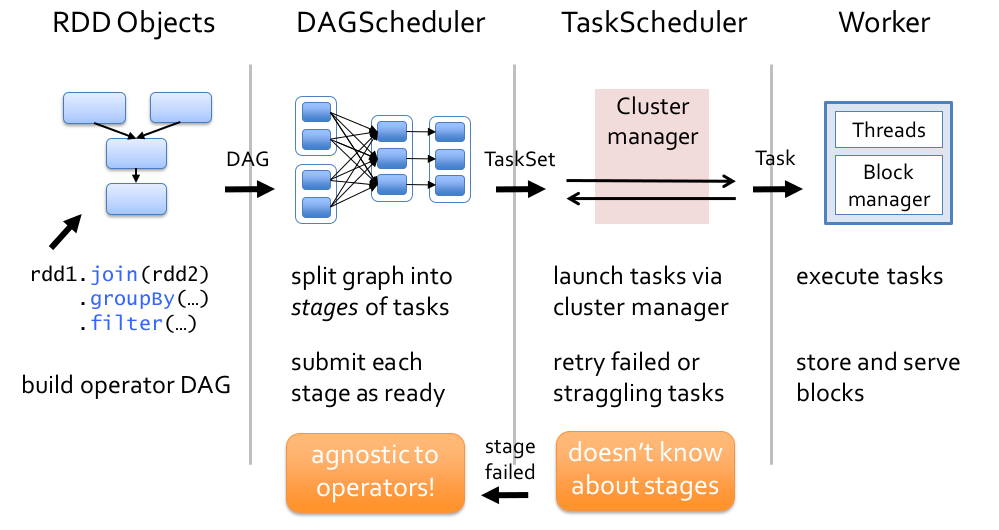
\includegraphics[width=\textwidth]{Figures/spark-job-lifetime.jpeg}
\caption{The lifetime of a Spark job}
\label{fig:lifetime}
\end{figure}

Figure \ref{fig:lifetime} illustrates those four steps clearly.

While the first three steps happen at the driver, the representation of the connection to the Spark cluster, the last step happens at the Executors. We go deeper into each step to understand a Spark Job Lifetime.\\

\textbf{RDD objects creation} Users create RDDs through a set of transformations, at the moment, the RDD is created at the driver.\\
\textbf{DAG Scheduling} When an action is called on an RDD, the RDD is transfered to the next step: DAG Scheduling. It is the process of splitting the DAG into stages, then submitting each stage as ready.
A module called DAGScheduler is in charge of DAG Scheduling. A stage is a set of independent tasks all computing the same function that need to run as part of a Spark job, where all the tasks have the same shuffle dependencies. Each DAG of tasks runs by the scheduler is splitted up into stages at the boundaries where shuffle occurs, and then the DAGScheduler runs these stages in topological order.\\
\textbf{Task Scheduling} TaskScheduler is the component which receives the stages from DAGScheduler and submits them to the cluster.\\
\textbf{Task Execution} Spark calls worker as Executor. The backend will receive the worker list from the Cluster Manager, then it will launchTask at the Executor. A BlockManager at each Executor will help it to deal with shuffle data and cached RDDs. New TaskRunner is created at the Executor and it starts the threadpool to process taskset, each task runs on one thread. After finishing the tasks, results are sent back to the driver or saved to disks.\\

Some information we need to notice are:
\begin{itemize}
\item Thanks to the DAGSchedulerEventProcessLoop, DAGScheduler can keep track of stages’ statuses and resubmit failed stages.
\item TaskScheduler only deals with taskSet after being formed from Stages at DAGScheduler,  that’s why it doesn’t know any thing about stages.
\item A Spark program can contain multiple DAGs, each DAG will have one action. So, inside a driver, they are submitted as jobs one by one in order.
\item Spark has a nice feature appears from version 1.2: dynamic resource allocation. Spark will base on the workload to request for extra resources when it needs or give the resources back to the cluster if they are no longer used.
\end{itemize}

\subsection{The Log Mining Example}

Below is an example about log mining. The idea of the example is loading the log, then we keep the error messages in memory and analyze it many times. By using caching, we can reduce the analyzed times. This is just a basic example to demonstrate how to write a Spark program, and the caching feature in action.

\begin{lstlisting}
//base RDD
val lines = spark.textFile("hdfs://...")

//transform to get error RDD, then cache it.
val errors = lines.filter(_.startsWith("ERROR"))
val messages = errors.map(_.split('\t')(2))
val cachedMsgs = messages.cache()

//action 1
cachedMsgs.filter(_.contains("foo")).count
//action 2
cachedMsgs.filter(_.contains("bar")).count
\end{lstlisting}

Table \ref{trans-act} gives us some basic transformations and actions inside Spark.\\

Firstly, create an RDD by reading an input file. Then we apply a set of transformations: filter and map to get the error logs and preprocessing them by splitting them by tabluture character. Then, we cache it. At the moment the "cache" command is called, nothing happens. When action 1 is happend, Spark keeps the cachedMsgs in memory, then filters the error logs which contains "foo". When action 2 is called, the cachedMsgs was kept in memory so Spark does not need to process everything from the beginning as the action 1 was called. If there are many actions after action 2 and they also process on cachedMsgs, they also do not need to process the previous part from scratch. This reduces the cost of I/O and computation many times.

%----------------------------------------------------------------------------------------
%	SECTION 2
%----------------------------------------------------------------------------------------

\section{Apache SparkSQL}
SparkSQL is a new module of Apache Spark, which provides the flexibilities for users to combine relational programming and functional programming through DataFrame API. It also provides an extensible optimizer called Catalyst, which utilizes the features of Scala language to make it easier to add new rules and to control code generation. The two following subsections brieftly describe these two contributions.\\


\subsection{DataFrame API}
DataFrames are distributed collection of column-structured records which can be manipulated by both new functional API and produceral API of Spark. DataFrames can be created from various data sources or even existing RDDs. 

DataFrame also provides user-defined function, which is very important for database systems. The inline-definition of UDFs also makes it easier for user to write their functions.\\
Each DataFrame object has a 'lazy' logical plan which means no execution occurs until an action is called, this let the logical plan itself have better chance of optimizations.\\ 

Spark SQL supports two different methods for converting existing RDDs into DataFrames:
\begin{itemize}
\item Using reflection to infer the schema of an RDD that contains specific types of objects. This method provides more concise codes and it works well when we already know about the schema of the object.
\item Using a programmatic interface, we can construct a schema and then apply it to an existing RDD. This method is more verbose, it allows us to construct DataFrames when the columns and their types are not known until runtime.
\end{itemize}

\subsection{Catalyst Optimizer}
Catalyst Optimizer is an extensible optimization engine. It contains a general library for representing trees and applying rules to manipulate them.\\
\textbf{Trees} Tree is the main data structure in Catalyst, which is formed by many nodes. A node has a type and its childs, which can be none or more than zero nodes. Node objects are read-only and can be manipulated using functional transformations.\\
\textbf{Rules} Trees can be transformed to another trees by using rules. By utilizing pattern matching, a Scala feature, a part of a tree can be found and replaced by another one.\\

\begin{figure}
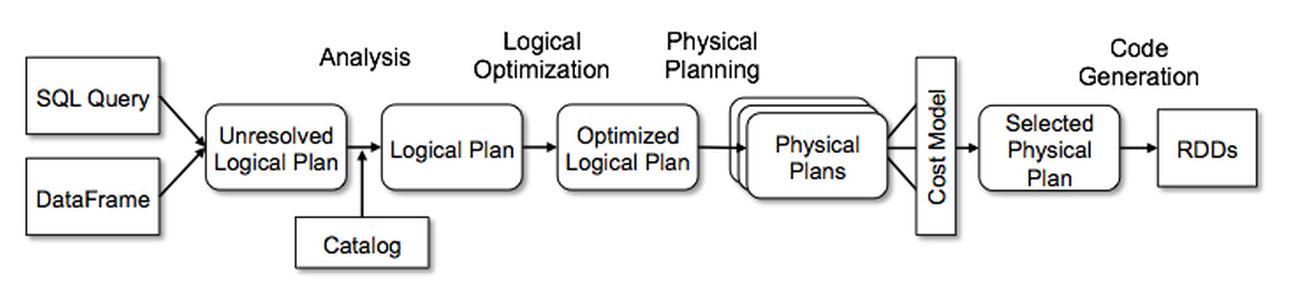
\includegraphics[width=\textwidth]{Figures/catalyst-flow.png}
\caption{Catalyst Dataflow}
\label{fig:catalyst1}
\end{figure}

A Catalyst tree transformation process is composed by four phases. Figure \ref{fig:catalyst1} illustrates this process. We explain each process below:
\begin{itemize}
\item \textbf{Analysis} Its input is a relation to be computed, which is created from SparkSQL Parser to form an Abstract Syntax Tree (AST) or from using DataFrame API. The relation can contain unresolved attribute references or relations, which means we do not know its type or have not matched it to an input table (or an alias). With Catalyst Rules and a Catalog, an object which is used to keep track of created tables, SparkSQL resolves those attributes.
\item \textbf{Logical Optimizations} This phase applies rule-based optimizations to the logical plan which is outputed from Analysis phase. By utilizing the nature of Scala language,users can simply add rules to fulfill their needs.
\item \textbf{Physical Planning} In this phase, Spark SQL tries to generate as much physical plans as possible from one optimized logical plan, by using physical operators that match the Spark execution engine. By associating to a cost model, it can select the best plan.
\item \textbf{Code Generation} This final phase of query optimization involves generating Java bytecode to run on each machine. By utilizing a special feature of Scala, which is quasiquotes, Catalyst can make code generation simpler. Quasiquotes allow the programmatic construction of abstract syntax trees (ASTs) in the Scala language, which can then be fed to the Scala compiler at runtime to generate bytecode. Again, due to the simplicity of quasiquotes, users can add their own rules for new types of expressions.
\end{itemize}
\subsection{An application written using SparkSQL}
Below is a simple example of SparkSQL to demonstrate the combination of relational programming and functional programming of SparkSQL.\\

\begin{lstlisting}
case class Person(name: String, age: Integer)
val input = sc.textFile("examples/src/main/resources/people.txt")
val people = input.map(_.split(",")).map(p => Person(p(0), p(1).trim.toInt))
val peopleDF = people.toDF()
peopleDF.registerTempTable("people")
val teenagers = sqlContext.sql("SELECT name FROM people WHERE age >= 13 AND age <= 19")
val result = teenagers.map(t => "Name: " + t(0)).collect.foreach(println)
\end{lstlisting}

We can declare our data structure, then read the input file with that format and store into an RDD. We create a DataFrame from that RDD and create a table from it. We are using the method of reflection to interoperate between DataFrame and RDD. An SQL query is passed to SparkSQL. After the optimization and translation happened, a normal Spark Job is created with a Directed-Acyclic Graph inside. An action would trigger all these things.

\begin{table}[]
\centering
\caption{Some transformatios and actions in Spark}
\label{trans-act}
\begin{tabular}{|l|l|}
\hline
\multicolumn{2}{|l|}{Transformation}           \\ \hline
\multicolumn{2}{|l|}{map(f : $T \Rightarrow $U) : $RDD[T] \Rightarrow $RDD[U]} \\ \hline
\multicolumn{2}{|l|}{filter(f : $T \Rightarrow $Bool) : $RDD[T] \Rightarrow $RDD[T]} \\ \hline
\multicolumn{2}{|l|}{flatMap(f : $T \Rightarrow $Seq[U]) : $RDD[T] \Rightarrow $RDD[U]} \\ \hline
\multicolumn{2}{|l|}{sample(fraction : Float) : $RDD[T] \Rightarrow $RDD[T]} \\ \hline
\multicolumn{2}{|l|}{groupByKey() : $RDD[(K, V)] \Rightarrow $RDD[(K, Seq[V])]} \\ \hline
\multicolumn{2}{|l|}{reduceByKey(f : $(V, V) \Rightarrow $V) : $RDD[(K, V)] \Rightarrow $RDD[(K, V)]} \\ \hline
\multicolumn{2}{|l|}{union() : $(RDD[T], RDD[T]) \Rightarrow $RDD[T]} \\ \hline
\multicolumn{2}{|l|}{join() : $(RDD[(K, V)], RDD[(K, W)]) \Rightarrow $RDD[(K, (V, W))]} \\ \hline
\multicolumn{2}{|l|}{cogroup() : $(RDD[(K, V)], RDD[(K, W)]) \Rightarrow $RDD[(K, (Seq[V], Seq[W]))]} \\ \hline
\multicolumn{2}{|l|}{crossProduct() : $(RDD[T], RDD[U]) \Rightarrow $RDD[(T, U)]} \\ \hline
\multicolumn{2}{|l|}{mapValues(f : $V \Rightarrow $W) : $RDD[(K, V)] \Rightarrow $RDD[(K, W)]} \\ \hline
\multicolumn{2}{|l|}{sort(c : Comparator[K]) : $RDD[(K, V)] \Rightarrow $RDD[(K, V)]} \\ \hline
\multicolumn{2}{|l|}{partitionBy(p : Partitioner[K]) : $RDD[(K, V)] \Rightarrow $RDD[(K, V)]} \\ \hline
\multicolumn{2}{|l|}{Actions} \\ \hline
\multicolumn{2}{|l|}{count() : $RDD[T] \Rightarrow $Long} \\ \hline
\multicolumn{2}{|l|}{collect() : $RDD[T] \Rightarrow $Seq[T]} \\ \hline
\multicolumn{2}{|l|}{reduce(f : $(T, T) \Rightarrow $T) : $RDD[T] \Rightarrow $T} \\ \hline
\multicolumn{2}{|l|}{lookup(k : K) : $RDD[(K, V)] \Rightarrow $Seq[V]} \\ \hline
\multicolumn{2}{|l|}{save(path : String) : Outputs RDD to a storage system, e.g., HDFS} \\ \hline

\end{tabular}
\end{table}